\documentclass[12pt, a4paper]{mycoursepaper}
\usepackage[a4paper,left=2.5cm,right=2cm,top=2cm,bottom=2cm,includefoot]{geometry}
\usepackage[utf8]{inputenc}
\usepackage[T1]{fontenc}
\usepackage[brazilian]{babel}
\usepackage{graphicx}
\usepackage{indentfirst}
\usepackage{array}
\usepackage{amsmath}
\usepackage{float}
\usepackage{multicol}
\usepackage{fancyhdr} 
\usepackage[usenames, dvipsnames]{color}
\usepackage[framed,numbered,autolinebreaks,useliterate]{mcode}
\usepackage{url,textcomp}
\usepackage[hidelinks]{hyperref}

\title{T03 Generate Random Data}
\author{Ricardo A. Fernandes}
\studentnumber{Matrícula: 2019105350 (PPGEC/CTEC/UFAL)}
\date{\today}
\college{Universidade Federal de Alagoas - UFAL\\
Instituto de Computação - IC\\
Programa de Pós-Graduação em  Informática - PPGI}
\coursename{Tópicos Especiais em Computação Visual e Inteligente: Aprendizagem Profunda}
\coursenumber{PPGI017-10}
\coursesection{-}
\instructor{Professor Tiago F. Vieira}

\newcommand{\norm}[1]{\lVert#1\rVert_2}

\begin{document}
\maketitle

\section{Gereção de Dados Randômicos}% \addtocounter{section}{1}
\vspace{-3mm}
Objetivo: Gerar dados randômicos de duas classes ``+'' e ``o'' usando numpy e matplotlib conforme ilustrado na Figura~\ref{fig:example}.
\vspace{-3mm}
\begin{itemize}
	\item use np.random.seed(1) para fixar a semente randômica e gerar distribuições mais próximas possíveis da Figura~\ref{fig:example}.
	\item Classe ``o'' tem média [0, 0].
	\item Classe ``+'' tem média [3, 4].
\end{itemize}
\vspace{-3mm}
\begin{figure}[H]
\centering
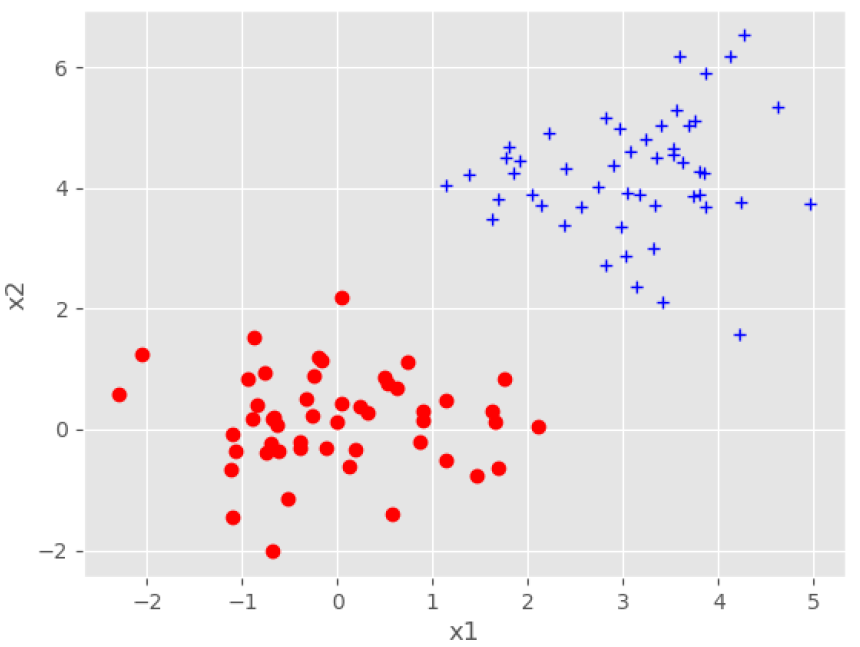
\includegraphics[width=0.45\paperwidth]{./example.png}
\caption{Ilustração das distribuições fornecidas para as classes ``o'' e ``+''.}
\label{fig:example}
\end{figure}

\newpage
\subsection{Resolução}
Desenvolveu-se a rotina generate\_random\_data.py (ver Listing~\ref{lst:grd}) em que se define a classe ``Data'' que recebe em seu construtor: nome, média e símbolo. A classe ``Data'' implementa também o método ``generate\_random\_sample'' que recebe um número de amostras e retorna dois arrays: $xs$ e $ys$. O método ``random.normal'' da numpy é utilizado para gerar os arrays $xs$ e $ys$, distribuições normais referentes às médias recebidas em cada direção, considerando desvio padrão unitário e o número de amostras fornecido.

Dessa forma, são criados os objetos $c$ e $p$, instâncias de ``Data'', representando as classes ``+'' e ``o'', respectivamente. Conforme orientação, utiliza-se a semente randômica 1 e chama-se o método ``generate\_random\_sample'' para ambos os objetos considerando 50 amostras. Os arrays retornados são plotados usando matplotlib, levando-se em consideração os nomes e símbolos previamente definidos.

% \lstinputlisting{../hellodl/generate_random_data.py}
\begin{lstlisting}[language=Python, caption=Rotina em Python3: generate\_random\_data.py, label=lst:grd]
import numpy as np
import matplotlib.pyplot as plt


class Data:  # define Data class
    def __init__(self, name, mean, mark):
        self.name = name,
        self.mean = mean
        self.mark = mark

    def generate_random_sample(self, n_samples):
        xs = np.random.normal(self.mean[0], 1, n_samples)
        ys = np.random.normal(self.mean[1], 1, n_samples)
        return xs, ys


c = Data('o', [0, 0], 'ro')  # circle instance
p = Data('+', [3, 4], 'b+')  # plus instance

# lock random seed
np.random.seed(1)

# generate samples
xc, yc = c.generate_random_sample(50)
xp, yp = p.generate_random_sample(50)

# plot samples
plt.plot(xc, yc, c.mark, label=c.name)
plt.plot(xp, yp, p.mark, label=p.name)

# set options and show plot
plt.xlabel('x1'), plt.ylabel('x2'), plt.grid(True)
plt.legend(loc='lower right')
plt.show()
\end{lstlisting}

\newpage
\subsection{Comparação entre as distribuições}

A Figura~\ref{fig:myrandomdata} ilustra as distribuições obtidas através da rotina generate\_random\_data.py utilizando o procedimento supracitado. Visualmente, observa-se boa concordância entre as distribuições geradas (ver Figura~\ref{fig:myrandomdata}) e as fornecidas (ver Figura~\ref{fig:example}).

\begin{figure}[H]
\centering
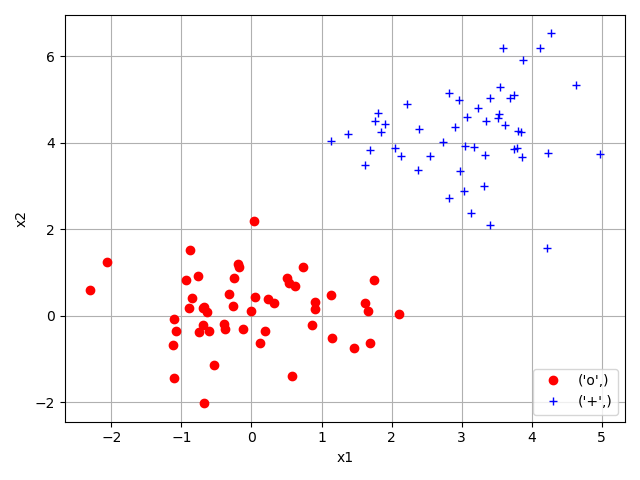
\includegraphics[width=0.45\paperwidth]{./myrandomdata.png}
\caption{Ilustração das distribuições geradas para as classes ``o'' e ``+''.}
\label{fig:myrandomdata}
\end{figure}

\begin{figure}[H]
\centering
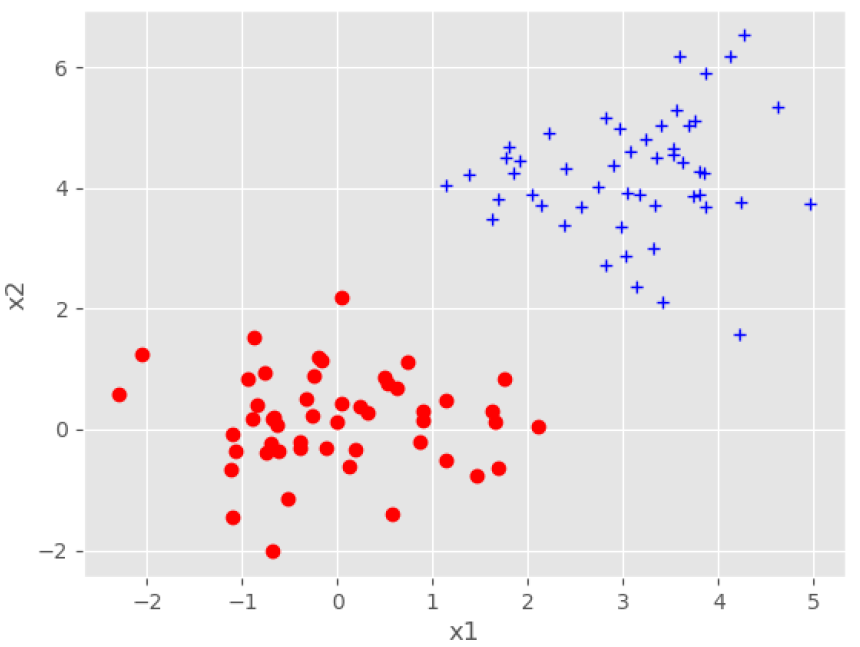
\includegraphics[width=0.45\paperwidth]{./example.png}
\caption{Ilustração das distribuições fornecidas para as classes ``o'' e ``+''.}
\label{fig:example}
\end{figure}



% Considere uma viga de comprimento $L$ com um carregamento $q_0$ uniformemente distribuído e com seção transversal retangular de base $b$ e altura $h$. Aplica-se uma força de protensão $f_0$ através de um cabo parabólico com excentricidade e no meio do vão (ver Figura~\ref{fig:viga}). Assumir valores numéricos para os parâmetros geométricos $L$, $b$ e $h$, para o módulo de elasticidade $E$ do material, para o carregamento $q_0$ e para as restrições laterais impostas. Considerar a força de protensão $f_0$ e a excentricidade $e$ como variáveis de projeto e utilizar o método gráfico para resolver o seguinte problema de otimização:
% \begin{subequations}
% \begin{alignat}{4}
% &\!\min_{f_0, e} &\qquad& f_0\label{eq:optProb1}\\
% &\text{s.t.} & & \sigma_L \leq \sigma \leq \sigma_U,\label{eq:constraint1}\\
% & & & \delta_L \leq \delta \leq \delta_U,\label{eq:constraint2}\\
% & & & e_L \leq e \leq e_U,\label{eq:constraint3}\\
% & & & f_0 \geq 0.\label{eq:constraint4}
% \end{alignat}
% \end{subequations}

% \begin{figure}[H]
% \centering
% \includegraphics[width=0.6\paperwidth]{./figuras/viga-crop.pdf}
% \caption{Viga protendida submetida a carregamento uniforme.}
% \label{fig:viga}
% \end{figure}

% \subsection{Cabo de protensão parabólico}

% Adotando o sistema de coordenadas mostrado na Figura~\ref{fig:parabola}, o cabo de protensão assume uma configuração parabólica dada por
% \begin{equation}
% y = a_0 + a_1 x + a_2 x^2.
% \label{eq:parabola}
% \end{equation}

% \begin{figure}[H]
% \centering
% \includegraphics[width=0.6\paperwidth]{./figuras/parabola-crop.pdf}
% \caption{Sistema de coordenada para representação da parábola.}
% \label{fig:parabola}
% \end{figure}

% Usando os pontos conhecidos na equação~(\ref{eq:parabola}),
% \begin{align}
% y\left(0\right) &= 0\\
% y\left(\frac{L}{2}\right) &= e\\
% y\left(L\right) &= 0,
% \end{align}
% e resolvendo as equações para as indeterminações $a_0$, $a_1$ e $a_2$, a configuração parabólica do cabo de protensão é determinada como
% \begin{equation}
% y = \frac{4 e}{L} x - \frac{4 e}{L^2} x^2.
% \label{eq:parabola_final}
% \end{equation}

% \subsection{Tensão longitudinal máxima}

% A tensão longitudinal máxima ocorre no meio do vão que representa a seção de maior momento fletor,
% \begin{equation}
% M_{q_0} = \frac{q_0 L^2}{8}.
% \end{equation}

% Admitindo que a força de protensão é perpendicular à seção da viga em suas extremidades, com base na equação~(\ref{eq:parabola_final}) da parábola, a carga equivalente $q_{f_0}$ à força de protensão $f_0$ pode ser determinada como
% \begin{equation}
% q_{f_0} = \frac{\text{d}^2 M_{f_0}}{\text{d} x^2} = f_0 \frac{\text{d}^2 y}{\text{d} x^2} = -\frac{8 e}{L^2} f_0,
% \label{eq:carga_f0}
% \end{equation}
% resultando no momento fletor $M_{f_0}$,
% \begin{equation}
% M_{f_0} = \frac{q_{f_0} L^2}{8} = -f_0 e.
% \end{equation}

% Considerando a área da seção transversal $A$ constante e o módulo $S$ de resistência à flexão para seção retangular dado por
% \begin{equation}
% S = \frac{b h^2}{6},
% \end{equation}
% e assumindo tensões positivas para tração e negativas para compressão, a tensão longitudinal máxima pode ser determinada por:
% \begin{align}
% \sigma &= \sigma_{f_0} + \sigma_{q_0}\\
% &= -\frac{f_0}{A} \pm \frac{1}{S}\left[M_{f_0}^\text{max} + M_{q_0}^\text{max}\right]\\
% &= -\frac{f_0}{b h} \pm \frac{6}{b h^2} \left[M_{q_0} + M_{f_0}\right]\\
% &= -\frac{f_0}{b h} \pm \frac{6}{b h^2} \left[\frac{q_0 L^2}{8} - f_0 e\right].
% \label{eq:tensao}
% \end{align}

% Visto que o carregamento $q_0$ induz tração nas fibras de baixo e compressão nas fibras de cima da viga e que a força de protensão $f_0$ gera um esforço normal de compressão, a tensão longitudinal máxima nas fibras de cima e de baixo da viga são dadas, respectivamente, por
% \begin{align}
% \sigma^t &= -\frac{f_0}{b h} - \frac{6}{b h^2} \left[\frac{q_0 L^2}{8} - f_0 e\right],\label{eq:tensao_t}\\
% \sigma^b &= -\frac{f_0}{b h} + \frac{6}{b h^2} \left[\frac{q_0 L^2}{8} - f_0 e\right].\label{eq:tensao_b}
% \end{align}


% \subsection{Deflexão máxima da viga}

% Devido às condições de contorno empregadas, a deflexão máxima da viga também ocorre no meio do vão. A deflexão máxima devido ao carregamento $q_0$ é dada por
% \begin{equation}
% \delta_{q_0} = \frac{5 q_0 L^4}{384 EI}.
% \end{equation}

% Utilizando a carga equivalente $q_{f_0}$ da equação~(\ref{eq:carga_f0}),
% determina-se a deflexão no meio do vão devido à força de protensão $f_0$ de forma semelhante,
% \begin{equation}
% \delta_{f_0} = \frac{5 q_{f_0} L^4}{384 EI}.
% \end{equation}

% Assim, calculando o momento de inércia de área de uma seção retangular,
% \begin{equation}
% I = \frac{b h^3}{12},
% \end{equation}
% a deflexão máxima do meio do vão é dada por
% \begin{align}
% \delta &= \delta_{q_0} + \delta_{f_0}\\
% &= \frac{5 L^4}{384 EI} \left[q_0 + q_{f_0}\right]\\
% &= \frac{5 L^4}{32 E b h^3} \left[q_0 - \frac{8}{L^2} f_0 e\right].
% \label{eq:deflexao}
% \end{align}

% \subsection{Problema de otimização}

% Com base nas expressões calculadas para a tensão longitudinal e deflexão máximas na viga, substituindo as equações~(\ref{eq:tensao_t}) e (\ref{eq:tensao_b}) em (\ref{eq:constraint1}) e a equação~(\ref{eq:deflexao}) em (\ref{eq:constraint2}), obtém-se
% \begin{subequations}
% \begin{alignat}{5}
% &\!\min_{f_0, e} &\qquad& f_0\label{eq:optProb1_new}\\
% &\text{s.t.} & & \sigma_L \leq -\frac{f_0}{b h} \pm \frac{6}{b h^2} \left[\frac{q_0 L^2}{8} - f_0 e\right] \leq \sigma_U,\label{eq:constraint1_new}\\
% & & & \delta_L \leq \frac{5 L^4}{32 E b h^3} \left[q_0 - \frac{8}{L^2} f_0 e\right] \leq \delta_U,\label{eq:constraint2_new}\\
% & & & e_L \leq e \leq e_U,\label{eq:constraint3_new}\\
% & & & f_0 \geq 0.\label{eq:constraint4_new}
% \end{alignat}
% \end{subequations}
% ou ainda, expressando as restrições na forma
% \begin{equation}
% g_i(f_0, e) \leq 0,
% \end{equation}
% tem-se
% \begin{subequations}
% \begin{alignat}{9}
% &\!\min_{f_0, e} &\qquad& f_0\label{eq:optProb1_new2}\\
% &\text{s.t.} & & g_{1,2}: -\frac{f_0}{b h} \pm \frac{6}{b h^2} \left[\frac{q_0 L^2}{8} - f_0 e\right] - \sigma_U \leq 0,\label{eq:constraint12_new2}\\
% & & & g_{3,4}: \frac{f_0}{b h} \mp \frac{6}{b h^2} \left[\frac{q_0 L^2}{8} - f_0 e\right] + \sigma_L \leq 0,\label{eq:constraint34_new2}\\
% & & & g_5: \frac{5 L^4}{32 E b h^3} \left[q_0 - \frac{8}{L^2} f_0 e\right] - \delta_U \leq 0,\label{eq:constraint5_new2}\\
% & & & g_6: -\frac{5 L^4}{32 E b h^3} \left[q_0 - \frac{8}{L^2} f_0 e\right] + \delta_L \leq 0,\label{eq:constraint6_new2}\\
% & & & g_7: e - e_U \leq 0,\label{eq:constraint7_new2}\\
% & & & g_8: -e + e_L \leq 0,\label{eq:constraint8_new2}\\
% & & & g_9: -f_0 \leq 0.\label{eq:constraint9_new2}
% \end{alignat}
% \end{subequations}

% É possível linearizar o problema de otimização ao se considerar a minimização nas variáveis $f_0$ e $m$. Dessa forma, além da substituição $m = f_0 e$ nas equações~(\ref{eq:constraint12_new2})-(\ref{eq:constraint6_new2}), as restrições $g_7$ e $g_8$ seriam reescritas na forma
% \begin{align}
% g_7&: m - f_0 e_U \leq 0\\
% g_8&: -m + f_0 e_U \leq 0.
% \end{align}

% No entanto, ao se optar pela solução gráfica do problema, essa linearização não é necessária, visto que um procedimento força bruta é empregado em sua resolução. Além disso, ao se resolver o problema de otimização através de solução gráfica, as restrições $g_7$, $g_8$ e $g_9$ que são restrições laterais nas variáveis de projeto não são mais necessárias, visto que é gerada uma malha de pontos com valores de $f_0$ e $e$ que já atendem a essas restrições.

% \subsection{Definição numérica do problema}

% Adotam-se os seguintes valores numéricos para o problema descrito:
% \begin{itemize}
% 	\item Comprimento do vão livre, $L = 12$ m
% 	\item Seção transversal, $b = 10$ cm e $h = 1$ m
% 	\item Carregamento uniforme, $q_0 = 20$ kN/m
% 	\item Módulo de elasticidade, $E = 30$ GPa
% \end{itemize}

% Para os valores limites de tensão e deflexão, assume-se:
% \begin{itemize}
% 	\item Restrição em tensão, $\sigma_L = -15$ MPa e $\sigma_U = 1$ MPa
% 	\item Restrição em deflexão, $\delta_U = -\delta_L = L/300 = 4$ cm
% \end{itemize}

% Devido à utilização de uma solução gráfica para o problema de otimização, é necessário se impor um limite superior à força de protensão,
% \begin{itemize}
% 	\item Restrição para força de protensão, $f_{0U} = 5$ MPa
% \end{itemize}

% Considerando uma cobertura de 5 cm para a viga, define-se o limite para a excentricidade do cabo de protensão no meio do vão,
% \begin{itemize}
% 	\item Restrição para excentricidade, $e_L = 0$ e $e_U = (h-2 \times 5\text{ cm})/2 = 45$ cm
% \end{itemize}

% Com base em um conjunto finito de valores adotados para as variáveis de projeto, ao se considerar os incrementos $\Delta{f_0} = 1$ e $\Delta{e} = 0.005$,
% \begin{align}
% f_0 &= \begin{bmatrix}
% 0 & \Delta{f_0} & \ldots & f_{0U}
% \end{bmatrix}\\
% e &= \begin{bmatrix}
% e_L & \Delta{e} & \ldots & e_U
% \end{bmatrix}
% \end{align}
% gera-se uma malha de pontos proveniente da combinação dos valores de $f_0$ e $e$. Para cada um desses pontos, se avalia o valor da função objetivo. Determinam-se também os valores de tensão máxima longitudinal nas fibras de cima e de baixo da viga e de deflexão máxima, para facilitar a avaliação das restrições do problema.

% A definição do problema, conforme os dados e considerações supracitadas, é implementada em linguagem MATLAB (ver Seção~\ref{appendix:a}). Neste arquivo, ainda definem-se propriedades das variáveis de projeto e das restrições que serão utilizadas pelo módulo de solução gráfica, tais como cores e descrições.

% % \begin{lstlisting}
% % function prestress_beam

% % % Input data
% % L = 12; b = 0.1; h = 1.0; % m
% % q0 = 20.0; % kN/m
% % E = 30.0e+06; % kPa

% % % Input bounds
% % s = [-15 1]*1.0e+03; % kPa
% % u = L/300*[-1 1]; % m
% % cover = 0.05; % m

% % % Define mesh
% % f0max = 5.0e+03; % kN
% % emax = (h-2*cover)/2; % m
% % [f0, e] = meshgrid(0:1:f0max, 0:0.005:emax);

% % % Define beam maximum stress and deflection
% % sigma_top = - f0./(b*h) - 6/(b*h^2) * (q0/8*L^2 - f0.*e);
% % sigma_bottom = - f0./(b*h) + 6/(b*h^2) * (q0/8*L^2 - f0.*e);
% % displ = 5/(32*E*b*h^3)*L^4 * (q0 - 8/L/L*f0.*e);

% % % Objective function and constraints
% % f = f0;
% % g{1} = sigma_bottom - s(2);
% % g{2} = sigma_top - s(2);
% % g{3} = -sigma_bottom + s(1);
% % g{4} = -sigma_top + s(1);
% % g{5} =  displ - u(2);
% % g{6} = -displ + u(1);

% % % Set graphical parameters
% % opt.feasible_color = [0.5 0.5 0.5];
% % opt.variable_name = {'f_0', 'e'};
% % opt.constraint_color = {'r', 'g', 'b', 'm', 'c', 'y'};
% % opt.constraint_name = {'\sigma_b upper bound', '\sigma_t upper bound', ...
% %     '\sigma_b lower bound', '\sigma_t lower bound', ...
% %     '\delta upper bound', '\delta lower bound'};

% % % Call graphical solution
% % graphical_optimization(f0, e, f, g, opt);
% % \end{lstlisting}

% \subsection{Solução gráfica do problema de otimização}

% O desenvolvimento da rotina para solução gráfica teve como ponto de partida um código disponibilizado pelo Prof. Adeildo S. Ramos Junior, que foi adaptado para funcionar de maneira independente da definição do problema de otimização. Dessa forma, pode-se definir todo o problema de otimização a ser estudado e, por fim, fazer uma chamada à rotina de solução gráfica (ver Seção~\ref{appendix:b}), garantindo maior modularização e clareza de código, conforme apresentado na rotina prestress\_beam na Seção~\ref{appendix:a}.

% % \begin{lstlisting}
% % function graphical_optimization (x1, x2, f, g, opt)
% % ne = size(f); % number of evaluations
% % nc = length(g); % number of constraints

% % % Identify feasible region
% % rv = true(ne); for i = 1:nc, rv = rv & g{i}<=0; end; rv = sparse(rv);
% % if all(rv(:)==false), disp('No feasible region'); return, end

% % % Find minimum objective function values inside feasible region
% % fmin = min(f(rv)); im = find(f==fmin & rv==true); xmin = [x1(im) x2(im)];
% % fprintf('\nfmin = %g\nxmin:\n', fmin); fprintf('[%g %g]\n',xmin');

% % % Show feasible region
% % figure('Color','w'); hold on;
% % plot(x1(rv), x2(rv), 'o', 'MarkerEdgeColor', opt.feasible_color, ...
% %     'MarkerSize', .1, 'MarkerFaceColor', opt.feasible_color, ...
% %     'HandleVisibility','off');

% % % Show contour of active constraints
% % for i = 1:nc
% %     contour(x1, x2, g{i}, [0 0], 'LineColor',opt.constraint_color{i}, ...
% %         'DisplayName', opt.constraint_name{i});
% % end

% % % Show objective function at its minimum value
% % c = clabel(contour(x1, x2, f, [fmin fmin], 'k--', 'DisplayName', ...
% %     'objective fcn')); set(c,'HandleVisibility','off');

% % % Show solution points
% % plot(x1(im), x2(im),'ob', 'MarkerFaceColor','w', 'DisplayName','solution')

% % % Define axes labels, colormap and display legend
% % xlabel(opt.variable_name{1}); ylabel(opt.variable_name{2});
% % colormap default; set(legend(gca,'show'),'Location','best');

% % \end{lstlisting}

% Nessa rotina, com base nas avaliações das restrições para os pontos da malha gerada previamente, se identifica uma possível região viável do problema. Se houver um domínio viável de solução, se encontram os valores mínimos avaliados para a função objetivo que pertecem a este domínio, caracterizando a solução do problema. Um gráfico ilustrando a região viável, bem como os limites de validade das restrições impostas são mostrados para o usuário. Nesse gráfico, ainda são destacados os pontos de mínimo que foram identificados através da solução gráfica. Configurações do gráfico como as cores da região viável e dos limites das restrições, os nomes das variáveis de projeto e as descrições das restrições são recebidos pela rotina através da variável opt.

% Para o estudo de caso com os valores numéricos propostos, o resultado da solução gráfica do problema de otimização é mostrado na Figura~\ref{fig:result}. A solução encontrada refere-se aos valores de força de protensão $f_0 = 557$ kN e excentricidade $e = 0.45$ m, e consequentemente, a função objetivo tem o mesmo valor de $f_0$, já que ela própria era o foco da minimização. As restrições ativas foram os limites superiores para a excentricidade $e$ e para a tensão longitudinal nas fibras de baixo $\sigma^b$.

% \begin{figure}[H]
% \centering
% \includegraphics[width=0.6\paperwidth]{./figuras/result-crop.pdf}
% \caption{Resultado da solução gráfica para o problema de viga protendida.}
% \label{fig:result}
% \end{figure}

% \subsection{Implementação MATLAB: definição do problema}
% \label{appendix:a}

% \begin{lstlisting}
% function prestress_beam

% % Input data
% L = 12; b = 0.1; h = 1.0; % m
% q0 = 20.0; % kN/m
% E = 30.0e+06; % kPa

% % Input bounds
% s = [-15 1]*1.0e+03; % kPa
% u = L/300*[-1 1]; % m
% cover = 0.05; % m

% % Define mesh
% f0max = 5.0e+03; % kN
% emax = (h-2*cover)/2; % m
% [f0, e] = meshgrid(0:1:f0max, 0:0.005:emax);

% % Define beam maximum stress and deflection
% sigma_top = - f0./(b*h) - 6/(b*h^2) * (q0/8*L^2 - f0.*e);
% sigma_bottom = - f0./(b*h) + 6/(b*h^2) * (q0/8*L^2 - f0.*e);
% displ = 5/(32*E*b*h^3)*L^4 * (q0 - 8/L/L*f0.*e);

% % Objective function and constraints
% f = f0;
% g{1} = sigma_bottom - s(2);
% g{2} = sigma_top - s(2);
% g{3} = -sigma_bottom + s(1);
% g{4} = -sigma_top + s(1);
% g{5} =  displ - u(2);
% g{6} = -displ + u(1);

% % Set graphical parameters
% opt.feasible_color = [0.5 0.5 0.5];
% opt.variable_name = {'f_0', 'e'};
% opt.constraint_color = {'r', 'g', 'b', 'm', 'c', 'y'};
% opt.constraint_name = {'\sigma_b upper bound', '\sigma_t upper bound', ...
%     '\sigma_b lower bound', '\sigma_t lower bound', ...
%     '\delta upper bound', '\delta lower bound'};

% % Call graphical solution
% graphical_optimization(f0, e, f, g, opt);
% \end{lstlisting}

% \newpage
% \subsection{Implementação MATLAB: solução gráfica}
% \label{appendix:b}
% \begin{lstlisting}
% function graphical_optimization (x1, x2, f, g, opt)
% ne = size(f); % number of evaluations
% nc = length(g); % number of constraints

% % Identify feasible region
% rv = true(ne); for i = 1:nc, rv = rv & g{i}<=0; end; rv = sparse(rv);
% if all(rv(:)==false), disp('No feasible region'); return, end

% % Find minimum objective function values inside feasible region
% fmin = min(f(rv)); im = find(f==fmin & rv==true); xmin = [x1(im) x2(im)];
% fprintf('\nfmin = %g\nxmin:\n', fmin); fprintf('[%g %g]\n',xmin');

% % Show feasible region
% figure('Color','w'); hold on;
% plot(x1(rv), x2(rv), 'o', 'MarkerEdgeColor', opt.feasible_color, ...
%     'MarkerSize', .1, 'MarkerFaceColor', opt.feasible_color, ...
%     'HandleVisibility','off');

% % Show contour of active constraints
% for i = 1:nc
%     contour(x1, x2, g{i}, [0 0], 'LineColor',opt.constraint_color{i}, ...
%         'DisplayName', opt.constraint_name{i});
% end

% % Show objective function at its minimum value
% c = clabel(contour(x1, x2, f, [fmin fmin], 'k--', 'DisplayName', ...
%     'objective fcn')); set(c,'HandleVisibility','off');

% % Show solution points
% plot(x1(im), x2(im),'ob', 'MarkerFaceColor','w', 'DisplayName','solution')

% % Define axes labels, colormap and display legend
% xlabel(opt.variable_name{1}); ylabel(opt.variable_name{2});
% colormap default; set(legend(gca,'show'),'Location','best');

% \end{lstlisting}
\end{document}
